\chapter{Calibration}
\label{chap:calibration}

The differences between data and MC efficiencies for various object selections have to be corrected to achieve accurate signal and background predictions.
The efficiencies of individual object selections are measured in data and applied to the MC.

\section{Lepton Efficiency}
\label{sec:lepton_eff}

The electron and muon efficiencies are measured using a similar method to the ``tag-and-probe'' method described in Section~\ref{sec:idsf}.
For these measurements, the tag object is an electron (muon) object passing the tight ID described in Section~\ref{sec:pf_electrons} (Section~\ref{sec:pf_muons}) and matched to a SingleElectron (SingleMuon) trigger while the probe object is an PF electron (muon) without any ID applied.
The passing (failing) categories are defined by events with probes passing (failing) the ID definition in question (see Sections~\ref{sec:pf_electrons} and~\ref{sec:pf_muons} for details).
The electron (muon) scale factors are approximately unity with a flat 2\% (1\%) systematic uncertainty.


\section{Pileup Reweighting}
\label{sec:puweight}

The distribution of the number of pileup interactions inserted into MC events differ from the true pileup distribution, estimated from the measurement of instantaneous luminosity, beam intensity of each proton bunch, and the total cross section of proton inelastic scattering (69.2 $\textrm{mb}^{-1}$).

Figure~\ref{fig:pudist} shows the pileup distributions in data and MC and their ratio. 
Each simulation event has its weight multiplied by the value of the ratio evaluated at the number of true pileup interaction injected into the event.

\begin{figure}[htbp]
  \centering
  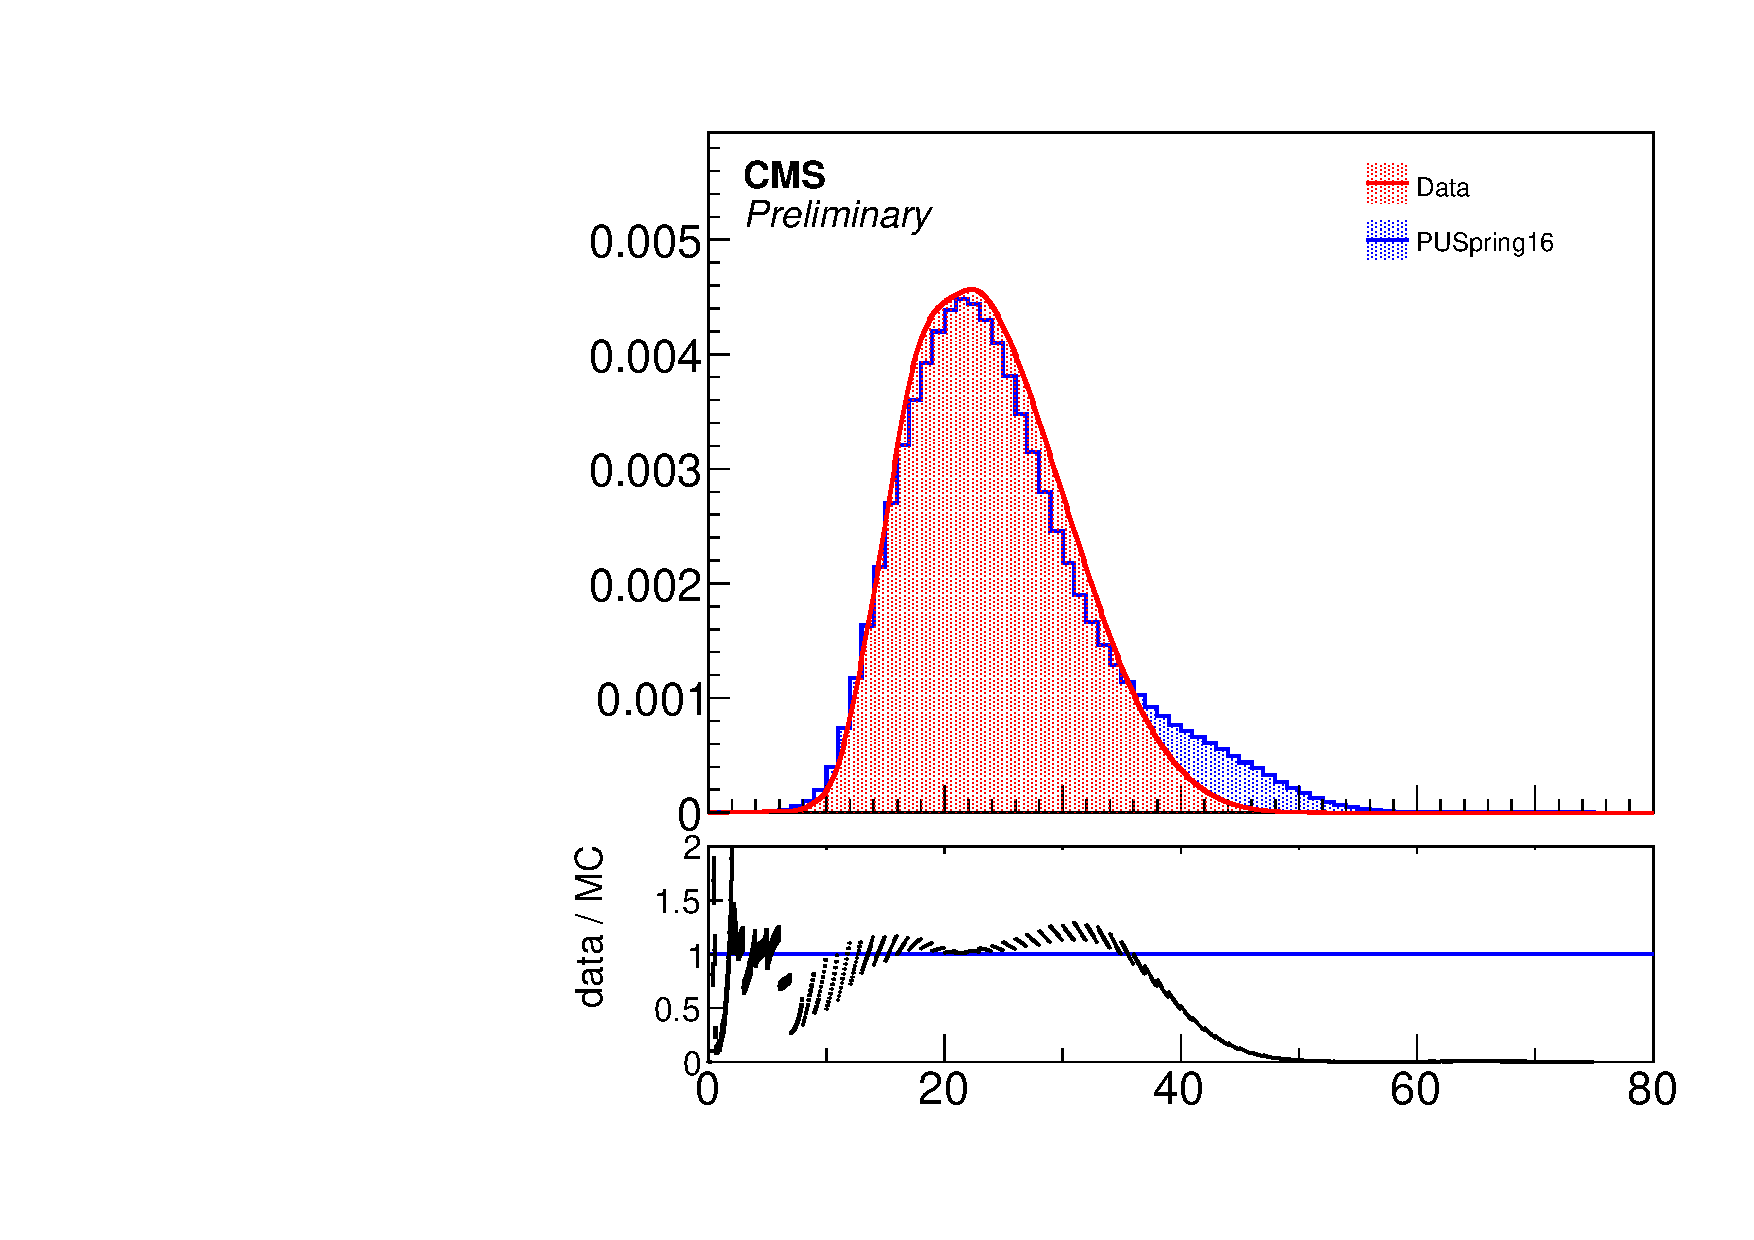
\includegraphics[width=0.48\linewidth]{Calibration/Figures/PUMoriond17.pdf}
  \caption{
    The pileup distributions in data and MC.
  }
  \label{fig:pudist}
\end{figure}

\section{Lepton Veto Efficiency (Events with ``Fake Leptons'')}
\label{sec:fake_lepton_veto}
The lepton veto requirement in the signal region has a non-unity efficiency over events that do not have genuine leptons, because particles such as pions and protons can mimic leptons (become ``fake leptons'') and cause the event to be rejected. 
To measure the possible difference between data and MC of this lepton veto efficiency, we compare dimuon events in data and MC. 
In a high-purity \Zmm\  sample with the dimuon mass close to $M_{\PZ}$, events with a genuine third lepton is negligibly rare, and therefore the efficiency loss from rejecting events with a third lepton is dominantly due to fake leptons.

For this measurement, collision events are taken from the SingleMuon data set and the MC events from a mixture of DY, \ttbar, \PW\PW, \PW\PZ, and \PZ\PZ\ samples. 
We require two muons passing the ``tight'' identification working point defined in Section~\ref{sec:pf_muons} with the mass between 61 and 121\GeV. 
These events are then checked for additional electron or muon objects passing the loose selection criteria defined in Sections~\ref{sec:pf_electrons} or~\ref{sec:pf_muons}, respectively. 
The efficiency is inspected as a function of number of vertices, number of jets, and $H_{\mathrm{T}}$ in the event, and in all cases data and MC are consistent as shown in Figure~\ref{fig:leptonveto_efficiencies}.

\begin{figure}[tbph]
 \centering
  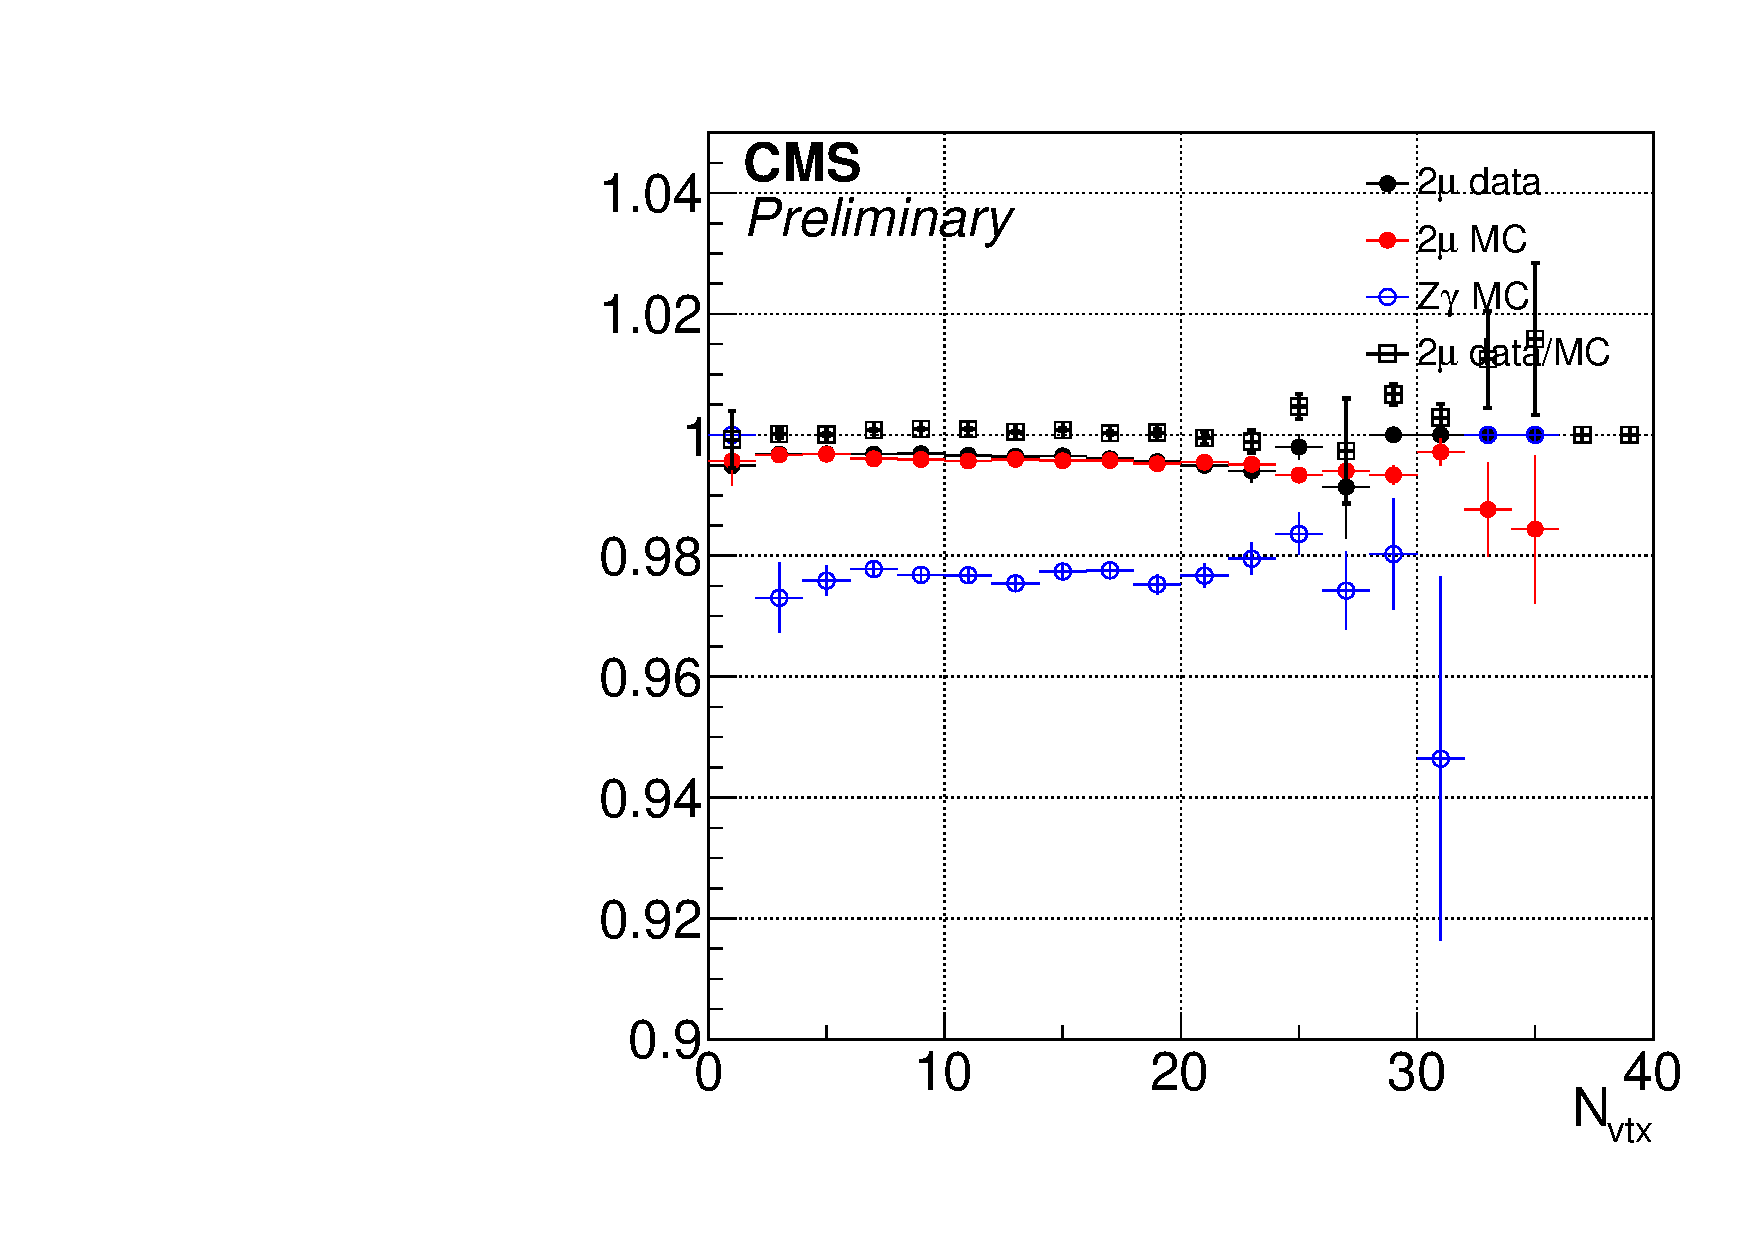
\includegraphics[width=7.5cm,height=7cm]{Calibration/Figures/leptonveto_eff_npv.pdf}
  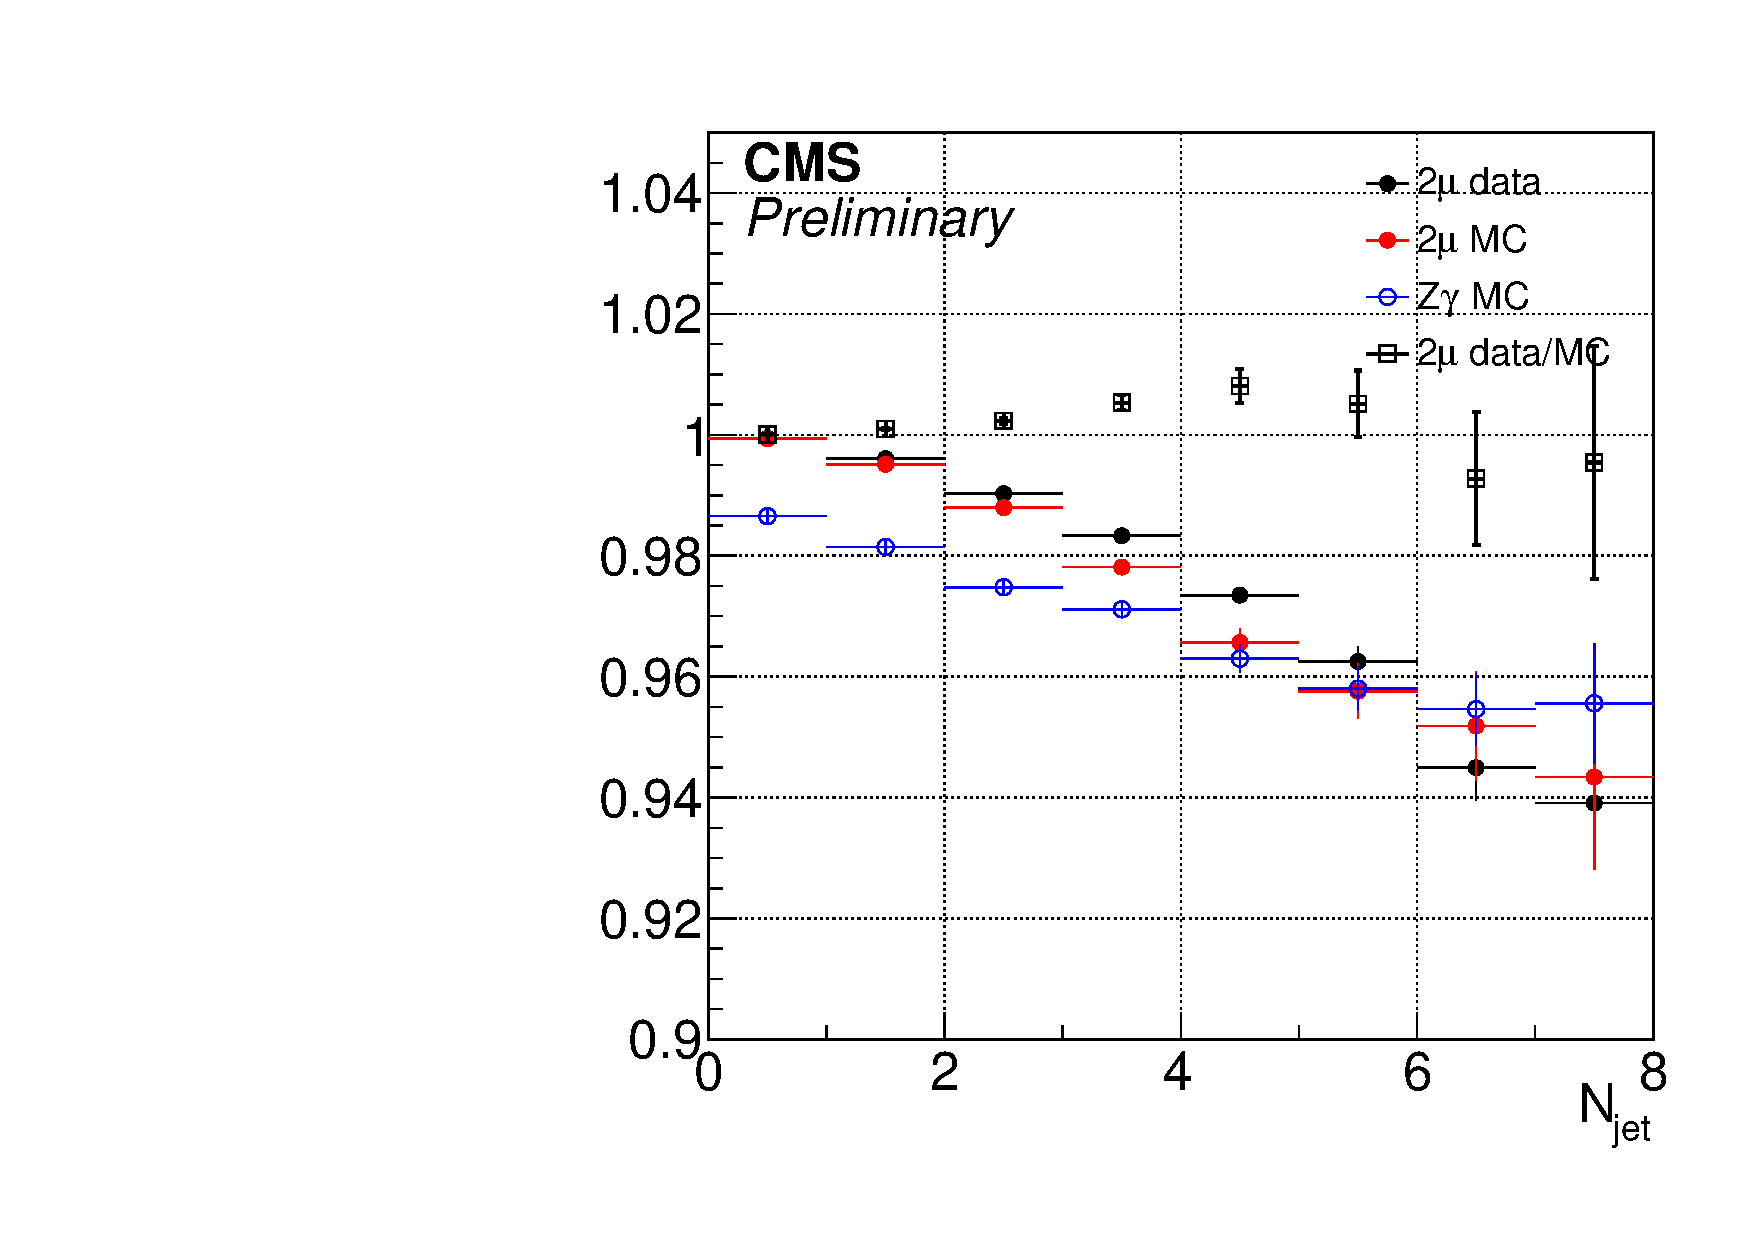
\includegraphics[width=7.5cm,height=7cm]{Calibration/Figures/leptonveto_eff_njet.pdf}
  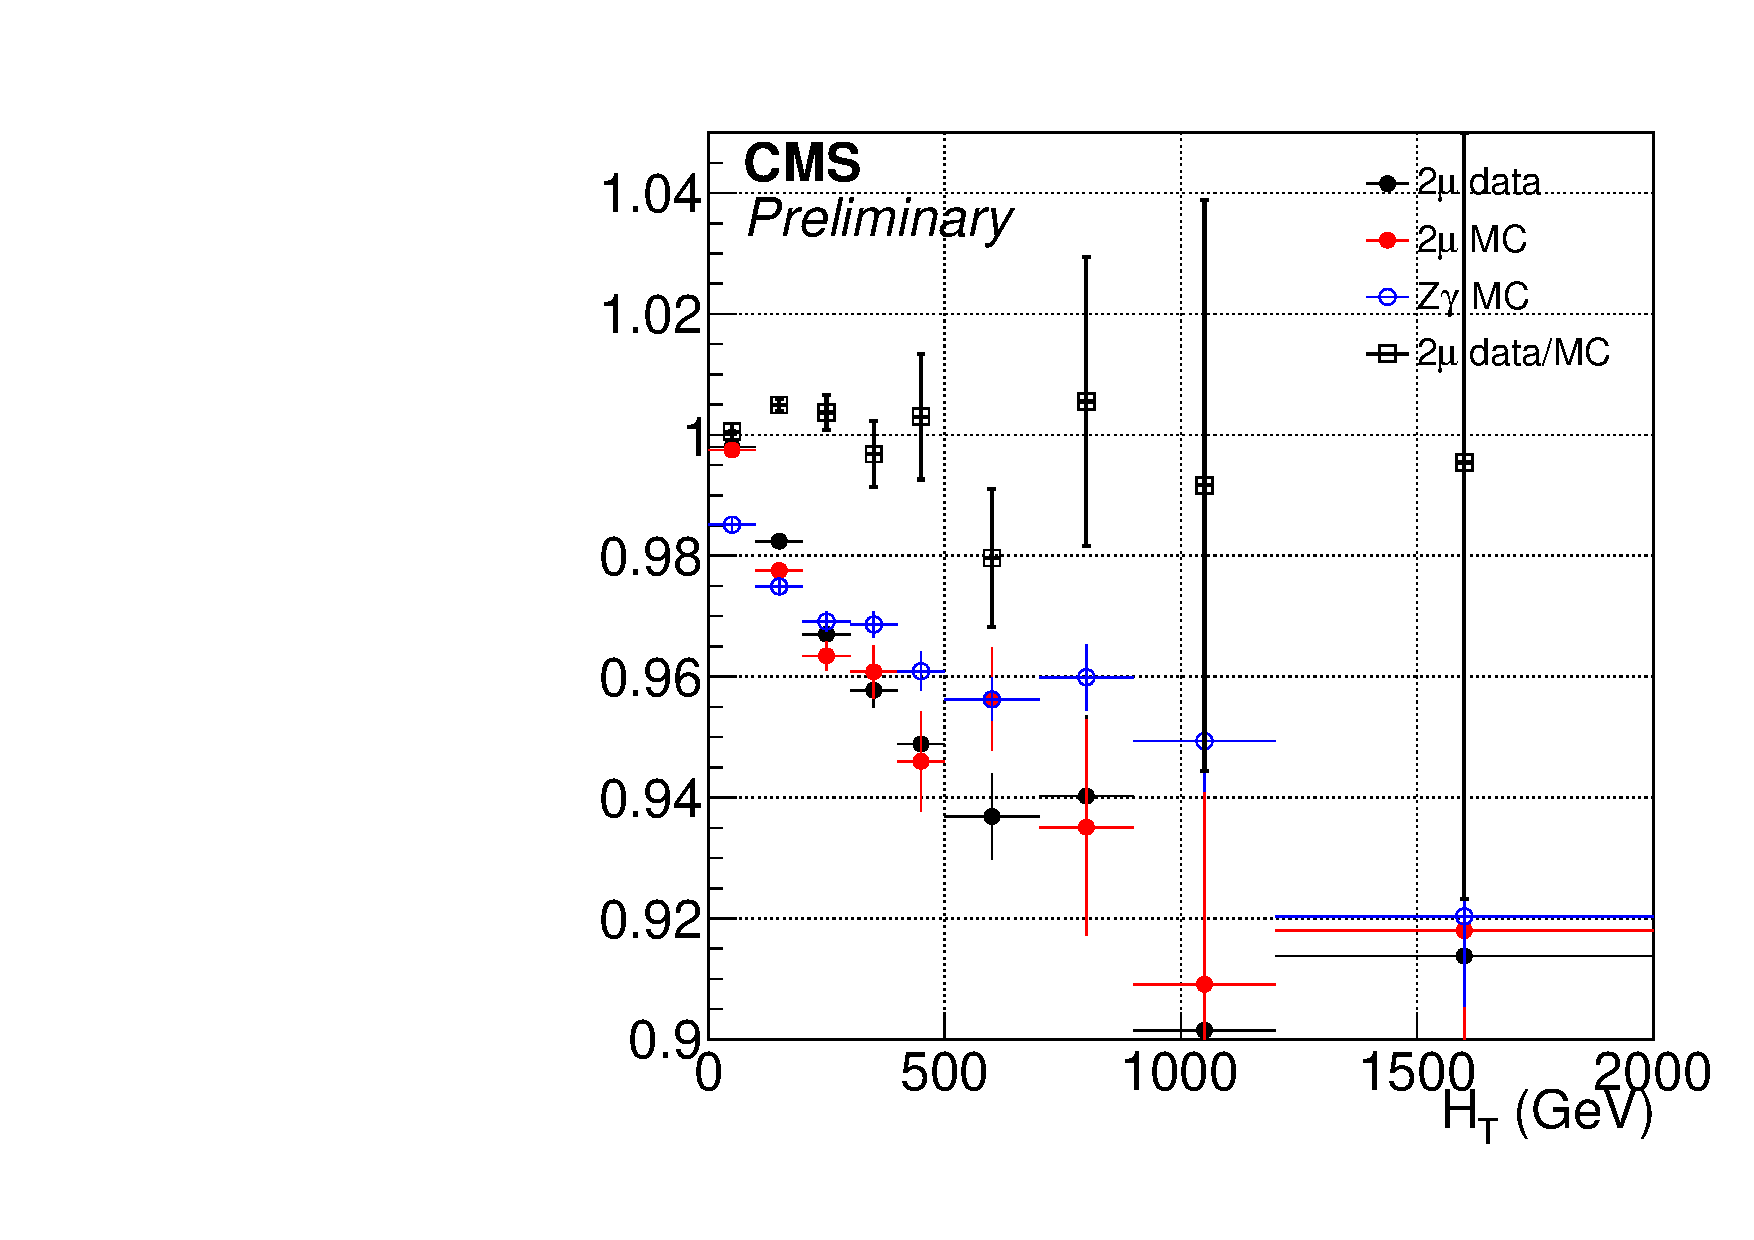
\includegraphics[width=7.5cm,height=7cm]{Calibration/Figures/leptonveto_eff_ht.pdf}
  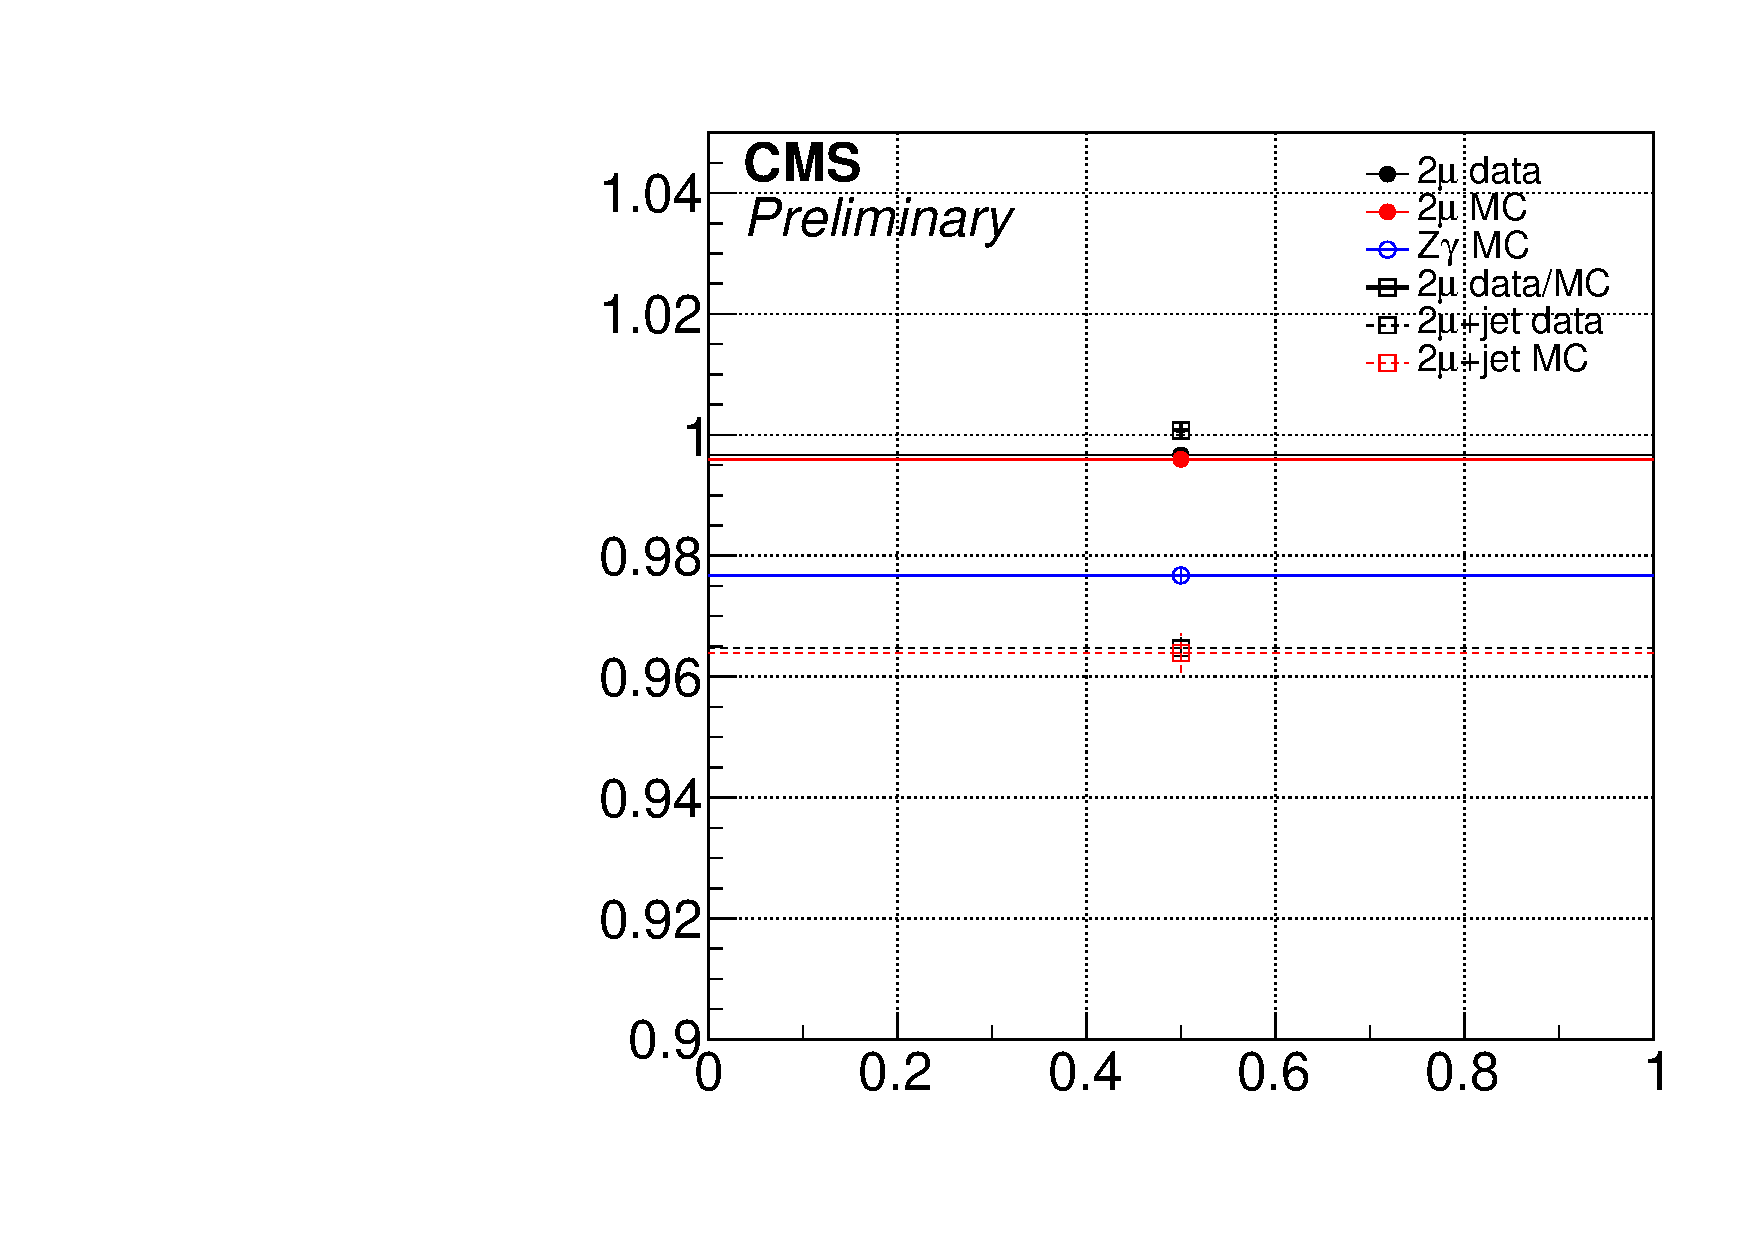
\includegraphics[width=7.5cm,height=7cm]{Calibration/Figures/leptonveto_eff_incl.pdf}
  \caption{
    Lepton veto efficiencies and data/MC scale factors as functions of $N_{\text{vtx}}$, $N_{\text{jet}}$, and $H_{\mathrm{T}}$, and the corresponding inclusive values. 
    While dimuon and \zinvg\ samples have significantly different efficiencies, data and MC agree well within dimuon samples, giving scale factors consisten with 1 almost everywhere. 
    This is true even when additionally requiring a high-\pt\ jet in the event, as seen in the inclusive efficiency plot. 
    Thus, the difference between \zinvg\ and dimuon efficiencies itself is taken as the uncertainty.
  }
 \label{fig:leptonveto_efficiencies}
\end{figure}

It should be noted, however, that the absolute lepton veto efficiency in MC dimuon sample is significantly different from that of the \zinvg\ sample, which more closely features the properties of the signal candidate sample. 
The full difference in the efficiencies between the dimuon and \zinvg\ samples is tentatively taken as the systematic uncertainty in the lepton veto scale factor, which is therefore $1.00 \pm 0.02$.

\section{Lepton Veto Efficiency (Events with ``Real Leptons'')}
\label{sec:real_lepton_veto}
Additionally, a small fraction of events with real leptons pass the lepton veto due to the leptons failing the loose ID requirements. 
This effect is most relevant for \wlng\ events in the signal region and for \zllg\ events in the single lepton control regions. 
We account for this effect in the following way:

Using the data and MC efficiencies from Section~\ref{sec:lepton_eff} for the loose IDs, we compute a scalefactor $\text{SF}_{\text{veto}} = (1. - \epsilon_{\text{data}}) / (1. - \epsilon_{\text{MC}})$ and apply  this to MC events with a reconstructed lepton that fails the loose ID. 
If there are multiple such  leptons in an event, we apply this scalefactor only for the hardest muon and electron. 
We apply a flat 1\% (5\%) uncertainty for the muon (electron) efficiencies. 

The veto scale factors for electrons (muons) range from 0.55 to 1.38 (0.34 to 73.5) with uncertainties  ranging from 0.15 to 1.46 (2.7 to 126.8). 
All scale factors are consistent with unity within the uncertainties. 
After applying the scale factors, the final MC yields for \wlng\ in the signal  region and \zllg\ in the single lepton control regions change by less than 0.5\%.
